\documentclass{article}
\usepackage[T1]{fontenc}
\usepackage{lmodern}
\usepackage{graphicx}
\usepackage{amsmath,amssymb}
\usepackage[a4paper,margin=2cm]{geometry}
\usepackage[absolute,overlay]{textpos}
\setlength{\TPHorizModule}{1mm}
\setlength{\TPVertModule}{1mm}
\usepackage[indonesian]{babel}
\usepackage{hyperref}
\setlength{\emergencystretch}{2em}
% unit: Halaman 53

\begin{document}

% === Halaman 53 (llm) ===

\vspace{119.99mm}

j = 0;\nfor (i=0; i<256; i++) {\n\t j = (j + S[i] + K[i \% K.length()]) \% 256;\n\t swap(S[i], S[j]); // Pertukarkan nilai S[i] dan S[j]\n}\n\ni = 0; j = 0;\nwhile (!leof(Fin)) {\n\t c = fgetc(Fin);\n\t i = (i + 1) \% 256;\n\t j = (j + S[i]) \% 256;\n\t swap(S[i], S[j]); // Pertukarkan nilai S[i] dan S[j]\n\t t = (S[i] + S[j]) \% 256;\n\t u = S[t]; // keystream\n\t p = u \^ c;\n\t fputc(p, Fout);\n}\nfclose(Fin); fclose(Fout);

% deskripsi: Potongan kode program implementasi algoritma RC4 dalam bahasa pemrograman C/C++.
% bbox normalisasi: [0.2140, 0.4600, 0.7670, 0.8640]
\begin{textblock*}{116.13mm}(44.94mm,136.62mm)
\noindent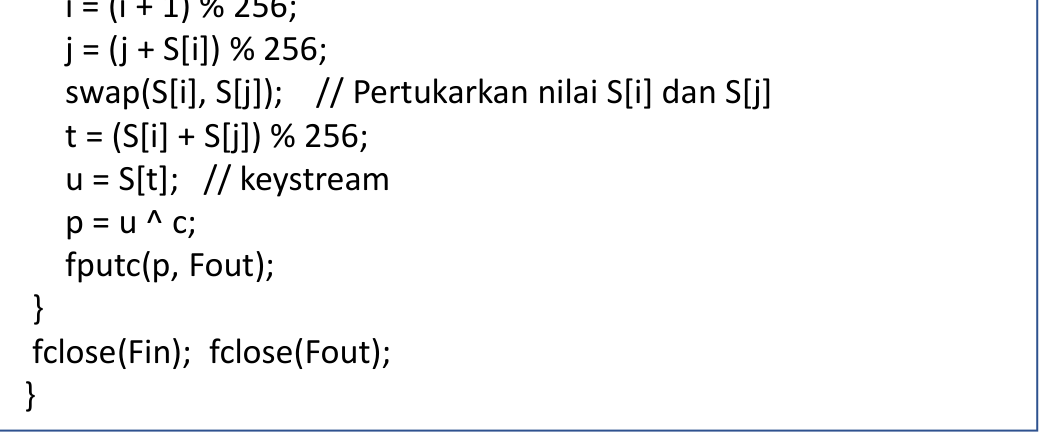
\includegraphics[width=116.13mm,height=119.99mm]{../../images/llm/page_053_img_01.png}%
\end{textblock*}

\end{document}
